\section{Разработка программных модулей}
\label{sec:develop_modules}

\subsection{Алгоритм расчета апостериорной вероятности для оценки стойкости шифрования}
\label{sub:develop_modules:k2_algorithm}

В данном подразделе рассматривается известный алгоритм, использующий оценку апостериорной вероятности в качестве критерия поиска стойкой тайны для шифрования данных.
Подробное описание данной оценки и базового алгоритма поиска приведены в работе~\cite{Cooper1991}.

Существуют подходы, использующие байесов метод для оценки качества полученной тайны и алгоритмы на их базе пытаются максимизировать апостериорную вероятность структуры шифра для данного набора экспериментальны данных.
В программном обеспечении, разработанном в данном дипломном проекте, использовался критерий оценки качества структуры, приведенный в упомянутой выше работе.

В данном подразделе рассматривается принцип минимальной длинны описания\footnote{В англоязычной литературе используется термин minimum description length или сокращенно MDL.} и его применимость для задания функции оценки качества шифра.
Данный принцип позволяет среди множества моделей выбрать модель с оптимальным соотношением сложности и соответствием модели наблюдаемым данным.
Т.\,е. данный принцип позволяет выбрать несложную и <<полезную>> модель, устойчивую к проблеме переобучения\footnote{В англоязычной литературе данная проблема называется overfitting и подразумевает, что модель слишком хорошо объясняет данные на которых она обучалась, но из-за этого непригодна для прогнозирования "--- работе на данных ранее не известных.}.
Принцип минимальной длинны описания в своей нестрогой и наиболее общей формулировке гласит: среди множества моделей следует выбрать ту, которая позволяет описать данные наиболее коротко, без потери информации~\cite{Grunwald05atutorial}.
Условие отсутствия противоречий модели во входном потоке является необходимым признаком адекватной модели, но не является достаточным. Простейшей моделью, удовлетворяющей такому условию, будет модель, в которой неопределенность, создаваемая неизвестными параметрами, очень велика и позволяет согласовать модель не только с реальными срезами потока, но вообще с любыми наборами величин. Во всех известных авторам реализациях существует одна и та же дилемма: чем больше количество параметров в модели, тем она точнее описывает совокупность данных, но тем ниже надежды на то, что такая модель окажется адекватной. При уменьшении же числа параметров модели, уменьшается и ее практическая значимость, поскольку такая модель гораздо менее точно описывает данные.

В контексте поиска модели стойкого шифра, соответствующей экспериментальным данным, принцип минимальной длинны описания гласит, что нужно выбрать модель, которая минимизирует сумму длин кодирования самой модели и кодирования экспериментальных данных с помощью этой модели~\cite{Lam94learningbayesian}, что выражается формулой~(\ref{eq:develop_modules:k2_algorithm:description_length}):
\begin{equation}
  \label{eq:develop_modules:k2_algorithm:description_length}
  l(x^{R}[n]) = \min_{g \in G}\left[ l_{G}(g) + l_{g}(x^{R}[n]) \right] \text{\,,}
\end{equation}
\begin{explanation}
где & $ x^R $ & вектор размерностью $R$, содержащий значения переменных (атрибутов). Представлен как $ x^R =\newline= (x^{(1)}, x^{(2)}, \dotsc, x^{(R)} ) $, где атрибут $ x^{(j)} $ может принимать $ \alpha_{j} $ значений, $ j = 1,\dotsc,R.$ \\
    & $ n $ & количество случаев в экспериментальных данных;  \\
    & $ x^R[n] $ & набор экспериментальны данных; \\
    & $ G $ & множество моделей; \\
    & $ l_{G}(g) $ & длина описания модели; \\
    & $ l_{g}(x^{R}[n]) $ & длина представления данных $ x^R[n] $ моделью $ g \in G $.
\end{explanation}

Для вычисления длинны кодирования модели и длинны кодирования данных с использованием модели в реализации дипломного проекта использовались результаты, приведенные в работах~\cite{Suzuki93,terentyev_2006}.
Собственно модель вероятностной сети состоит из таблиц условных и безусловных распределений и отношений <<родитель"=потомок>> между вершинами.
Для вычисления длины кодирования модели можно воспользоваться формулой~(\ref{eq:develop_modules:k2_algorithm:model_length}):
\begin{equation}
  \label{eq:develop_modules:k2_algorithm:model_length}
  l_{G}(g) = \frac{\log{n}}{2} \cdot \sum_{k = 1}^{R} S_k(g) (\alpha_k - 1) \text{\,,}
\end{equation}
\begin{explanation}
где & $ S_k(g) $ & количество возможных назначений переменных"=родителей переменной $X_k$, способ вычисления данного значения отличается у классических шифров и их модификации.
\end{explanation}

Введем некоторые обозначения, в дополнение к тем, которые были введены в подразделе~\ref{eq:develop_modules:k2_algorithm:description_length}.
Пусть структура шифра обозначается символом $B_S$, таблицы условных распределений, ассоциированные с ним, "--- $B_P$.
\newpage
Две вероятностные сети для данного набора экспериментальных данных можно оценить по отношению~(\ref{eq:develop_modules:k2_algorithm:nets_ratio}) апостериорных вероятностей:
\begin{equation}
  \label{eq:develop_modules:k2_algorithm:nets_ratio}
  \frac{P(B_{S_i} | x^R[n])}{P(B_{S_j} | x^R[n])} =
    \frac{ \frac{P(B_{S_i}, x^R[n])}{P(x^R[n])} }
         { \frac{P(B_{S_j}, x^R[n])}{P(x^R[n])} } =
    \frac{ P(B_{S_i}, x^R[n]) }
         { P(B_{S_j}, x^R[n]) } \text{\,.}
\end{equation}

Как видно из приведенной формулы~(\ref{eq:develop_modules:k2_algorithm:nets_ratio}), научившись вычислять отношение совместных распределений, можно сравнивать апостериорные вероятности структур вычисляемых шифров.
Т.\,к. в разработанном ПО использовались результаты, приведенные в работе~\cite{Cooper1991}, то считаем целесообразным привести в данном подразделе базовые формулы и предположения из вышеупомянутой работы.

Для вычисления $P(B_S, D)$ важно сделать несколько важных предположений:

\begin{enumerate}
  \item
  Экспериментальные данные содержат только дискретные случайные величины и все эти случайные величины присутствуют в истинной структуре $B_S$ модели из которой были получены эти экспериментальные данные.
  Из данного предположения следует формула~(\ref{eq:develop_modules:k2_algorithm:assumption1}):
  \begin{equation}
    \label{eq:develop_modules:k2_algorithm:assumption1}
    \int_{B_P} P(x^R[n] | B_S, B_P) f(B_P | B_S) P(B_S) dB_p \text{\,,}
  \end{equation}
  \par\hspace{\fivecharsapprox} % абзацный отступ
  \begin{tabular}{@{}ll@{ --- }p{0.74\textwidth}}
  где & $ B_P $ & вектор, содержащий значения условных вероятностей для назначений переменных из структуры $ B_S $; \\
      & $ f $ & условная плотность распределения $B_P$ при условии структуры $B_S$. \\[\parsep]
  \end{tabular}

  \item
  Случаи, зафиксированные в экспериментальных данных, независимы друг от друга, при условии зафиксированной модели, т.\,е. данное предположение подразумевает, что модель, генерирующая экспериментальные данные не меняется.
  Это предположение позволяет упростить формулу~(\ref{eq:develop_modules:k2_algorithm:assumption1}) и привести её к виду:
  \begin{equation}
    \label{eq:develop_modules:k2_algorithm:assumption2}
    P(B_S, x^R[n]) =
      P(B_S) \int_{B_P} \left[ \prod_{j = 1}^{n} P(x^R_j | B_S, B_P) \right] f(B_P | B_S) dB_P \text{\,.}
  \end{equation}

  \item
  Экспериментальные данные не должны содержать пропущенных значений для переменных из структуры $B_S$.
  Введем дополнительные обозначения.
  Пусть $x_j^{(i)}$ представляет значение $i$-й переменной в $j$-м случае.
  Пусть $\phi_i$ представляет из себя вектор уникальных назначений переменных"=родителей для $i$-й переменной, т.\,е. вектор уникальных назначений для $ \forall X_k,\ k \in \pi_i$.
  Пусть $\sigma(i, j)$ индексная функция, которая возвращает индекс назначения $\pi_i$ в $j$-ом случае из вектора $\phi_i$.
  Введем обозначение для длинны вектора $q_i = | \phi_i |$.
  Теперь с учетом предположения об отсутствии пропущенных значений можно вычислить вероятность конкретного случая из экспериментальных данных по формуле:
  \begin{equation}
    \label{eq:develop_modules:k2_algorithm:case_prob}
    P(x^R_j | B_S, B_P) =
      \prod_{i = 1}^{R} = P(X_i = x_j^{(i)} | \phi_i[\sigma(i, j)], B_P) \text{\,.}
  \end{equation}
  Подставляя выражение~(\ref{eq:develop_modules:k2_algorithm:case_prob}) в формулу~(\ref{eq:develop_modules:k2_algorithm:assumption2}) получим:
  \begin{align}
    \label{eq:develop_modules:k2_algorithm:assumption3}
    P(B_S, x^R[n]) =
      P(B_S)
      \int_{B_P}\left[ \prod_{j = 1}^{n}\prod_{i = 1}^{R} P(X_i = x_j^{(i)} | \phi_i[\sigma(i, j)], B_P)  \right] &\times \notag\\
      \times f(B_P | B_S) dB_P \text{\,.}
  \end{align}
  Пусть для выбранных $i$ и $j$ $f(P(x_i | \phi_i[j], B_P))$ обозначает плотность распределения возможных значений $P(x_i | \phi_i[j], B_P)$.
  Необходимо сделать еще одно предположение.

  \item Для $ 1 \le i, i' \le n$, $ 1 \le j \le q_i $, $1 \le j' \le q_i $, если
  $ij \neq i'j'$, то распределение $f(P(x_i | \phi_i[j]))$ не зависимо от распределения $f(P(x_{i'} | \phi_{i'}[{j'}]))$.
  Данное предположение по свой сути полагает, что до того, как были получены экспериментальные данные, все возможные назначения равновероятны.
\end{enumerate}

С учетом приведенных выше предположений и теоремы, приведённой и доказанной в работе~\cite{Cooper1991}, можно привести формулу для вычисления $P(B_S, D)$:
\begin{equation}
  \label{eq:develop_modules:k2_algorithm:model_and_data_prob}
  P(B_S, x^R[n]) =
    P(B_S)
    \prod_{i = 1}^{R}
    \prod_{j = 1}^{q_i}
    \frac{(\alpha_i - 1)!}
         {(n[\phi_i[j], i, B_S] + \alpha_i - 1)!}
    \prod_{k = 1}^{\alpha_i}
      n[v_{ik}, \phi_i[j], i, B_S]! \text{\,,}
\end{equation}
\par
\begin{tabular}{@{}ll@{ --- }p{0.74\textwidth}}
где & $ v_{ik} $ & $k$-е возможное назначение переменной $X_i$. \\[\parsep]
\end{tabular}

Формула~(\ref{eq:develop_modules:k2_algorithm:model_and_data_prob}) позволяет вычислить значение $P(B_S, x^R[n])$, если известна вероятность $P(B_S)$ и подсчитана оставшаяся часть формулы на основе экспериментальны данных $x^R[n]$.
Но из-за того, что $P(B_S)$ является чаще неизвестной величиной, чем известной, предполагают, что все возможные структуры сети равновероятны и $P(B_S)$ является некой малой константой.
Апостериорную вероятность структуры можно вычислить по формуле~(\ref{eq:develop_modules:k2_algorithm:aposteriori_structure_given_data}):
\begin{equation}
  \label{eq:develop_modules:k2_algorithm:aposteriori_structure_given_data}
  P(B_S | x^R[n]) =
    \frac{P(B_S, x^R[n])}
         {\sum_{B_S}P(B_S, x^R[n])} \text{\,.}
\end{equation}

Но, как уже упоминалось, множество возможных структур слишком велико, и на практике значение апостериорной вероятности можно вычислить лишь для шифров данных малой длины.

Формулу~(\ref{eq:develop_modules:k2_algorithm:model_and_data_prob}) для оценки совместной вероятности на практике напрямую использовать не получится, без введения дополнительных предположений.
Необходимо сделать предположение, что все возможные структуры равновероятны, т.\,е. $P(B_S)$ равно некоторой малой константе $c$.
Таким образом нахождение оптимальной структуры сводится к максимизации формулы~(\ref{eq:develop_modules:k2_algorithm:optimization_objective}), т.\,e. задача сводится к нахождению множества вершин"=предков $ \pi_i $ для каждой вершины $X_i$, оптимизирующих целевую функцию~\cite{Cooper1991}.
\begin{align}
  \label{eq:develop_modules:k2_algorithm:optimization_objective}
  \max \left[ P(B_S, x^R[n]) \right] = \notag\\
  =
    c \prod_{i = 1}^{R} \max_{\pi_i}
    \bigg[
      \prod_{j = 1}^{q_i} &% to align formula
      \frac{(\alpha_i - 1)!}
           {(n[\phi_i[j], i, B_S] + \alpha_i - 1)!}
      \prod_{k = 1}^{\alpha_i}
        n[v_{ik}, \phi_i[j], i, B_S]!
    \bigg] \text{\,.}
\end{align}

Таким образом наивный алгоритм поиска состоит в полном переборе всех возможных родителей для каждой вершины и оптимизации при этом функции~(\ref{eq:develop_modules:k2_algorithm:node_optimization_obj}):
\begin{equation}
  \label{eq:develop_modules:k2_algorithm:node_optimization_obj}
  g(i, \pi_i) =
    \prod_{j = 1}^{q_i}
      \frac{(\alpha_i - 1)!}
           {(n[\phi_i[j], i, B_S] + \alpha_i - 1)!}
      \prod_{k = 1}^{\alpha_i}
        n[v_{ik}, \phi_i[j], i, B_S]! \text{\,.}
\end{equation}

На практике наивный вариант не годится из-за большого количества возможных вариантов структур шифров.
В разработанной реализации использовались те же ограничения и стратегия поиска, что и в работе~\cite{Cooper1991}.
Перед началом выполнения алгоритма требуется знание о порядке вершин, таком, что вершины родители всегда находятся раньше вершин потомков.
Схематически алгоритм поиска выглядит следующим образом:

\begin{lstlisting}[style=fsharpstyle,escapeinside={/*@}{@*/},caption={Псевдокод реализации алгоритма К2}, label=lst:arch_and_mod:k2_algorithm:k2_pseudo]
function k2 =
  (* Input: dataset $x^R[n]$, ordering of variables, u - maximum number of parents per variable.
     Output: for each node, a printout of the parents of the node. *)
  for i in 1 .. R do
    $ \pi_i $ := $ \emptyset $
    $P_{old}$ := $g(i, \pi_i)$; // formula(/*@\ref{eq:develop_modules:k2_algorithm:node_optimization_obj}@*/)
    OkToContinue := true;
    while OkToContinue and $|\pi_i| < u$ do
      let z = node in $ \text{Pred}(X_i) - \pi_i $ that maximizes $ g(i, \pi_i \cup {z}) $
      $P_{new}$ := $f(i, \pi_i \cup {z})$
      if $P_{new} > P_{old}$ then
        $P_{old}$ := $P_{new}$;
        $ \pi_i $ := $ \pi_i \cup {z} $
      else OkToContinue := false
    end while
    printfn("Node: ", $X_i$, "Parents of $X_i$:", $\pi_i$)
  end for
end
\end{lstlisting}

В разработанной в рамках дипломного проекта реализации за основу был взят алгоритм К2, приведенный в работе~\cite{Cooper1991}, псевдокод которого показан в листинге~\ref{lst:arch_and_mod:k2_algorithm:k2_pseudo}.
В разработанном алгоритме слегка изменен способ подсчета целевой функции.
Приняв во внимание ограничение задания на дипломное проектирование, а также то, что операции умножения, деления и возведения в степень более сложные, было принято решение воспользоваться прологарифмированной версией формулы~(\ref{eq:develop_modules:k2_algorithm:node_optimization_obj}).

В качестве оценки степени зависимости двух произвольных переменных в работе~\cite{Chow68approximatingdiscrete} было предложено использовать значение взаимной информации\footnote{В англоязычной литературе используется термин mutual information}.
Эта информация задаёт приоритет поиска зависимостей между переменными.
По своей сути значение обоюдной информации является аналогом корреляции, но по своему содержанию "--- это оценка количества информации содержащейся в одной переменной о другой~\cite{terentyev_2006}.
Значение взаимной информации принимает неотрицательные значения и равно нулю в случае независимости случайных величин.
Для вычисления взаимной информации была предложена формула~(\ref{eq:develop_modules:k2_algorithm:mutual_information}):
\begin{equation}
  \label{eq:develop_modules:k2_algorithm:mutual_information}
  I(X; Y) = \sum_{y \in Y} \sum_{x \in X}
                 p(x, y) \log{ \left(\frac{p(x, y)}{p(x)\,p(y)}
                              \right) } \text{\,,}
\end{equation}
\begin{explanation}
где & $ p(x, y)$ & совместное распределение случайных величин $X$ и $Y$; \\
    & $ p(y) $ & безусловное распределение случайной величины $X$; \\
    & $ p(x) $ & безусловное распределение случайной величины $Y$.
\end{explanation}

Ниже приводится точная формула~(\ref{eq:develop_modules:k2_algorithm:log_node_optimization_obj}), по которой вычисляется оценка в реализованном алгоритме на основании формулы~(\ref{eq:develop_modules:k2_algorithm:mutual_information}), предложенной в работе~\cite{Chow68approximatingdiscrete}.
Данная формула более удобная для вычисления на платформе разработки, указанной в задании на дипломное проектирование:
\begin{align}
  \label{eq:develop_modules:k2_algorithm:log_node_optimization_obj}
  \log(g(i, \pi_i)) &=
    \sum_{j = 1}^{q_i}
      \log
      \left(
        \frac{(\alpha_i - 1)!}
             {(n_{ij} + \alpha_{i} - 1)!}
        \prod_{k = 1}^{\alpha_i}
          n_{ijk}!
      \right) =\notag\\
    &=
    \sum_{j = 1}^{q_i}
      \left(
        \log
          \frac{(\alpha_i - 1)!}
               {(n_{ij} + \alpha_{i} - 1)!}
        +
        \log
          \prod_{k = 1}^{\alpha_i}
            n_{ijk}!
      \right) =\notag\\
    &=
    \sum_{j = 1}^{q_i}
      \left(
        \log (\alpha_i - 1)! - \log (n_{ij} + \alpha_{i} - 1)!
        +
        \sum_{k = 1}^{\alpha_i}
          \log n_{ijk}!
      \right) =\notag\\
    &=
      \sum_{j = 1}^{q_i}
      \left(
        \log \Gamma(\alpha_i) - \log \Gamma(n_{ij} + \alpha_{i})
        +
        \sum_{k = 1}^{\alpha_i}
          \log \Gamma(n_{ijk} + 1)
      \right) = \notag\\
    &=
      q_i \log \Gamma(\alpha_i) +
      \sum_{j = 1}^{q_i}
      \left(
        \sum_{k = 1}^{\alpha_i}
          \log \Gamma(n_{ijk} + 1)
        - \log \Gamma(n_{ij} + \alpha_{i})
      \right) \text{\,,}
\end{align}
\begin{explanation}
где & $ \Gamma $ & гамма-функция "---  расширение понятия факториала на поле комплексных чисел; \\
    & $ n_{ijk} $ & условное, более краткое, обозначение для $n[v_{ik}, \phi_i[j], i, B_S]$; \\
    & $ n_{ij} $ & условное, более краткое, обозначение для $n[\phi_i[j], i, B_S]$.
\end{explanation}

Помимо использования формулы~(\ref{eq:develop_modules:k2_algorithm:log_node_optimization_obj}) в реализации были произведены дополнительные оптимизации, продиктованные результатами профилирования реализации алгоритма, изложенные в подразделе~\ref{sub:develop_modules:class}.

\subsection{Классификатор нормализации данных}
\label{sub:develop_modules:class}

Класс \foreignlanguage{english}{Certificate} использует большие простые числа для формирования классификатора. Время обработки каждого члена классификатора, содержащего числа высокой разрядности затруднено проблемами факторизации~\cite{facto_number}. Для сокращения времени обработки и вычисления тайны, базовые операции компрессии и нормализации данных были разбиты на каскады простых операций, формализованных асинхронными методами.

Каскады объединяются в каскады классификаторов. Процесс анализа членов сводится к тому, что простые числа последовательно анализируется на каждом каскаде классификатора, получая уникальную порцию примеси и смещения. При этом на каждом этапе происходит отсеивание некоторого количества разрядов, которые на последующих стадиях обрабатываться уже не будут. После того, как тайна пройдет через все каскады классификатора, выдается результат.

Однако из-за того, что прототип тайны имеет фиксированный размер, каждый член классификатора был снабжен вторым уникальным хеш-ключем, который по размеру соответствуют анализируемой области. Для создания тайны произвольного размера применяется два подхода: либо масштабирование классификатора, либо масштабирование самой тайны.

Структуру классификатора, который используется в программе генерации тайны, графически можно изобразить как на рисунке~\ref{fig:develop_modules:class:class_default}.

\begin{figure}[ht]
\centering
  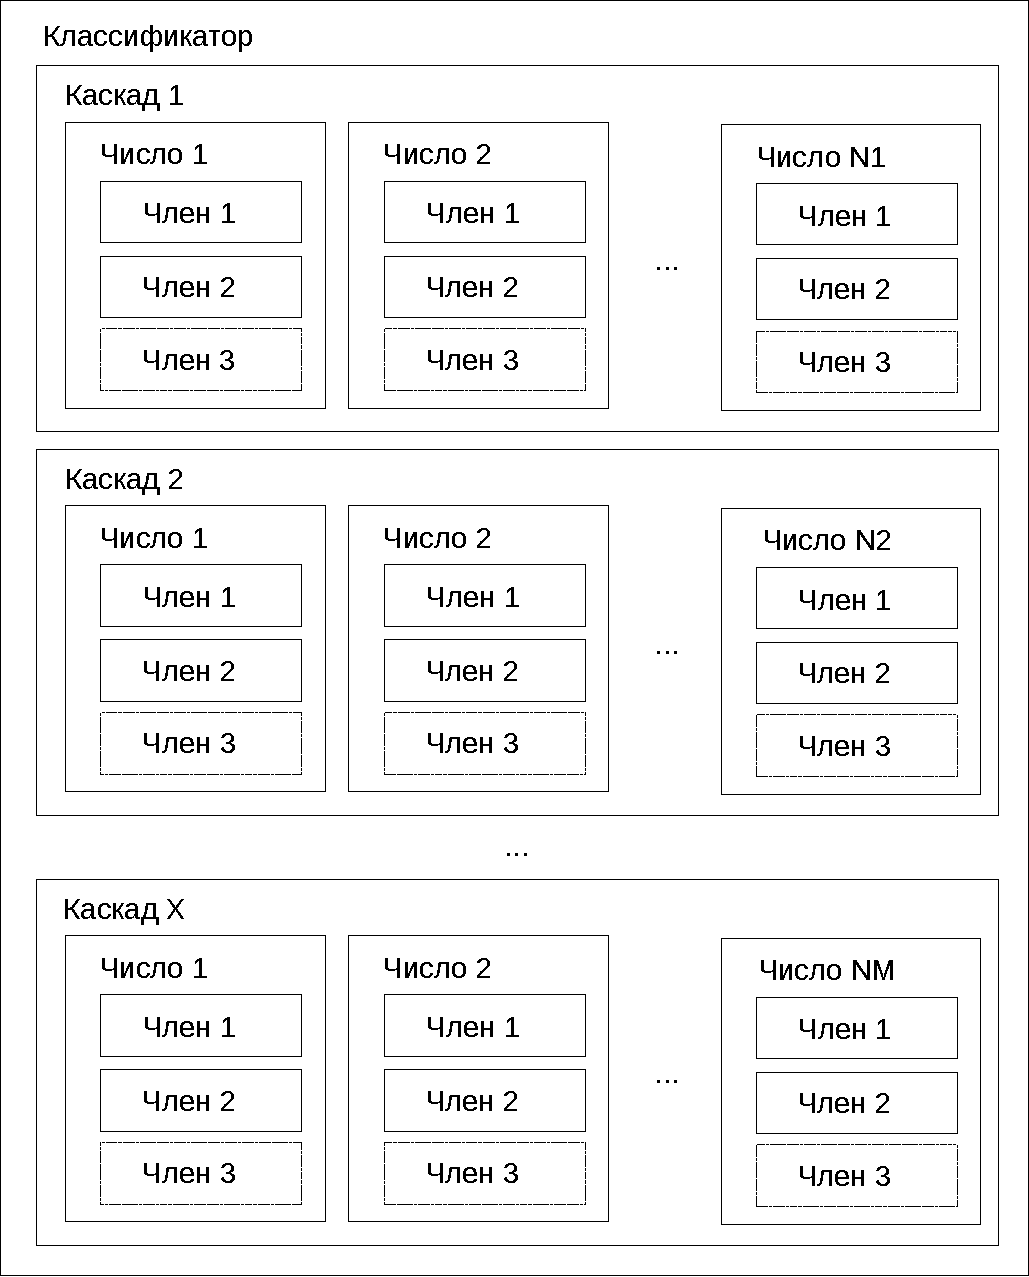
\includegraphics[scale=0.5]{class_default.pdf}
  \caption{ Структура классификатора. }
  \label{fig:develop_modules:class:class_default}
\end{figure}

Как видно из данного рисунка, классификатор состоит из множества каскадов, в каждый из которых входит набор чисел. Каждое число определяет два или три члена (так как третье член может отсутствовать, оно отмечено штрихом). Однако такая структура не является оптимальной, потому что она требует лишние операции над членами при работе. Поэтому была разработана структура, которая минимизирует число операций, на ряду с обфускацией связей между ними. Она изображена на рисунке~\ref{fig:develop_modules:class:class_changed}.

\begin{figure}[ht]
\centering
  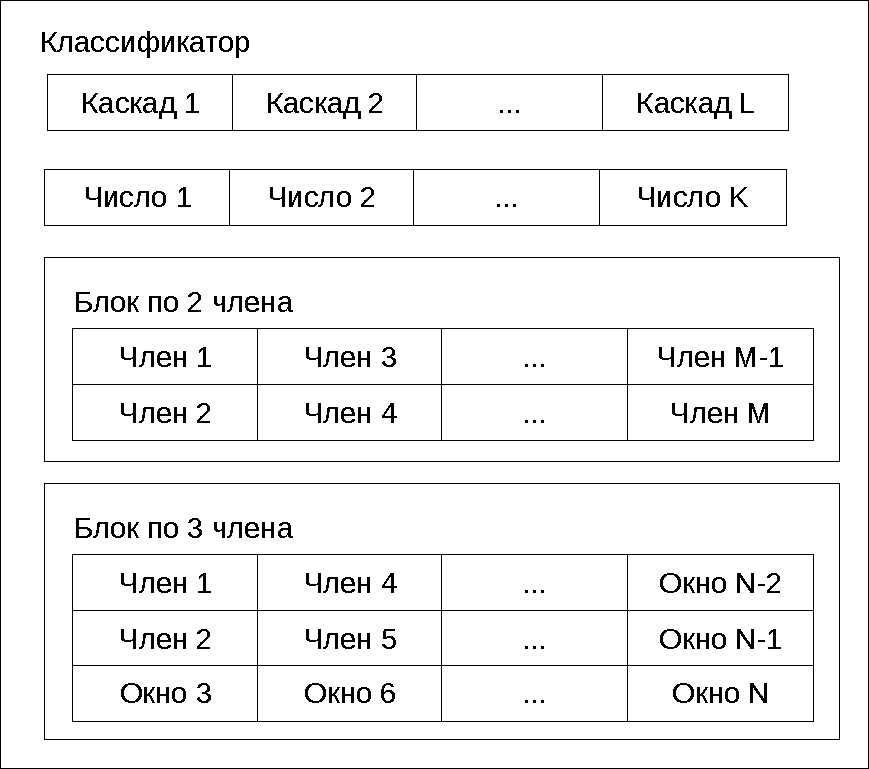
\includegraphics[scale=0.6]{class_changed.pdf}
  \caption{ Минимизированная структура классификатора }
  \label{fig:develop_modules:class:class_changed}
\end{figure}

\newpage

Для описания классификатора на рисунке~\ref{fig:develop_modules:class:class_changed} были разработаны следующие структуры:
\begin{lstlisting}[style=fsharpstyle,escapeinside={/*@}{@*/},caption={Структуры классификатора}, label=lst:develop_modules:class:structurs]
enum number_cascade {
  UInt32Array<number> node2_count,
  UInt32Array<number> node2_first,
  UInt32Array<number> node3_count,
  UInt32Array<number> node3_first,
  UInt32Array<number> node_position,
  Float32Array<number> threashold
};

enum number_rect {
  UInt8ClampedArray<number> p1,
  UInt8ClampedArray<number> p2,
  UInt8ClampedArray<number> p3,
  UInt8ClampedArray<number> p4
};

enum number_node {
  number a;
  number b;
  Float32Array<number> threashold;
};
\end{lstlisting}

Структура number\_cascade соответствует описанию каскадов. Так как все числа и члены располагаются линейно без разделения на каскады, структура должна содержать индексы начала блоков по два члена node2\_first, по три члена node3\_first и начало блока чисел node\_position. Также, чтобы упростить вычисления, введено число членов по два node2\_count и по три no"=de3\_count, количество чисел для данного каскада определяется как сумма блоков по два и три члена. Переменная threashold используется для принятия окончательного решения – подходит или нет данная область.
Все окна описывает структура number\_rect. Ее элементы описывают смещение относительно членов, который рассматривается в текущий момент данным вычислительным блоком.
Множеству чисел соответствует структура number\_node. Данная структура используется для наращивания порогового значения, на основе которого будет приниматься окончательное решение, на фиксированную величину в зависимости от результата сравнения простых чисел, полученного после обработки всех членов каскада, с эталонным значением данного числа threashold.

С учетом данных структур введены следующие переменные:

\begin{lstlisting}[style=fsharpstyle,escapeinside={/*@}{@*/},caption={Переменные данных структур}, label=lst:develop_modules:class:data_structurs]
const number_rect haar_rects2[ITEM2];
const haar_rect_weights2[ITEM2];
const number_rect haar_rects3[ITEM3];
const number_rect_weights3[ITEM3];
const number_node haar_nodes[NODES];
const number_cascade haar_cascade[CASCADES];
\end{lstlisting}

В них переменные ITEM2 и ITEM3 описывают максимальное число по два и три члена соответственно, NODES – количество чисел на все каскады, CASCADES – число каскадов, которые нужно обработать. Переменные haar\_rect\_weights2 и haar\_rect\_weights3 используются для хранения значения длины тайны.

Для обработки первых двух каскадов используется функция haar\_fir"=st\_stage. Эта функция обрабатывает простые числа каждого члена, что связано с нехваткой ресурсов, требуемых для обработки всех разрядов. Выходным значением данной функции является массив res\_number, который представляет собой сформированный шаблон тайны. Дополнительно для данной функции может применяться функция filter. В ее задачу входит модифицирование тайны таким образом, чтобы из нее был удален каждый второй подряд идущий элемент, а также преобразование блока обработки, так как последующие каскады работают только с членами типа UInt8Array.

После того как маска сформирована, управление передается модулю формирования тайны. В случае если тайна для пользователя готовится впервые, вызывается функция SecurityToKen. Член каскада представляет собой координаты единичных элементов в тайне. Члены каскада, которые ничего не обрабатывают, имеют пустое поле хеш-функции.

После этого осуществляется вызов функции для обработки очередного каскада классификатора. При этом последующие каскады уже должны поддерживать работу с предыдущими, а не с исходной маской смещения.
Такое разделение связано с тем, что член становится слишком разреженным и, несмотря на использование проверки, максимальной производительности добиться не удается~\cite{comp_security}, так как для значительного числа каскадов данных для обработки нет.  В случае, когда один член каскада обрабатывается двумя, четырьмя либо восемью каскадами, все множество чисел, которые требуется обработать для данного каскада, разделяются между данным числом каскадов равномерно, что позволяет оптимизировать нагрузку между вычислительными методами и добиться значительного ускорения.

После того, как будет обработан очередной каскад классификатора, управление передается функции DataToQueue. Она является аналогом функции SecurityToKen, но учитывает уже обработанные каскады. DataToQueue снова вызывается обработчик членов и цикл повторяется. Число каскадов, которые будут обрабатываться с применением DataToQueue передаются в нее после выполнения SecurityToKen. После того, как будут обработаны все каскады классификатора, вызывается функция RestoreMask. Ее основная задача сводится к тому, чтобы преобразовать значение членов каскадов, полученные после обработки их в DataToQueue, к типу, пригодному к обработке генератором. В частности, первый цикл событий обрабатывает последовательно каждый член каскада, а второй обрабатывает последовательно весь массив, не разбивая его на блоки. По результату выполнения каскада функция возвращает тайну пользователя, необходимую для получения нормализованных данных.